\lstset{
 upquote=true,
 showspaces=false,
 showtabs=false,
 frame=none,
 tabsize=2,
 breaklines=true,
 numbers=none,
 showstringspaces=false,
 breakatwhitespace=true,
 escapeinside={(*@}{@*)},
 keywordstyle=\bfseries,
 basicstyle=\footnotesize\ttfamily,
}

\section*{Lab activity 2}

\subsection*{Topology diagram}
\begin{figure}[htb]
	\centering
	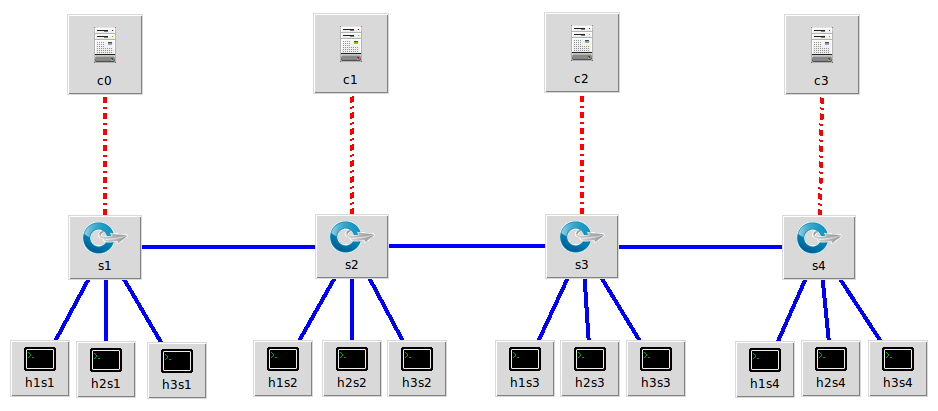
\includegraphics[width=1\linewidth]{img/topology-2.png}
	\caption{the topology that will be implemented during this lab activity.
  It is a linear topology with four switches connected to each other,
  each one connected to three hosts. Each switch is linked to a different
  SDN controller. All the controllers can be assumed local.}
	\label{fig:topology-2}
\end{figure}

\subsection*{Learning objectives}
After finishing this lab activity you will be able to:
\begin{itemize}
  \item create a custom switch class that extends the OVSSwitch class provided
  by the Mininet Python API
  \item implement a cluster of local/remote controllers inside Mininet using a custom
  switch class and the topology classes provided by the Mininet high-level API
  \item implement more complex topologies with multiple controllers using a
  few lines of Python code
  \item reflect upon the method used in this activity for implementing a cluster of controllers
  and compare it with the method shown in Activity 1, focusing on the advantages
  and disadvantages of each method
  \item test the network connectivity and the performance of a network with multiple
  controllers.
\end{itemize}






\subsection*{Scenario}
In this activity you will implement the topology shown in figure \ref{fig:topology-2} using
a Python script and the classes provided by the high-level Mininet API, which
represent topology templates. In order to use these classes for creating a network
with multiple controllers, you will have to define a new switch class that extends
the standard OVSSwitch class provided by the API.

Begin by creating a new Python script and importing the required Mininet classes.
Create the controllers shown in the topology diagram and define
a custom switch class which extends the class \code{OVSSwitch}. Define a function for creating
the network and inside its body use one of the topology templates provided
by the API to implement the required topology.
After writing the script, execute it and test the network connectivity and its
performance. To conclude, answer the questions proposed in the last task.

This lab activity assumes that:
\begin{itemize}
  \item you are proficient in SDN networks
  \item you are proficient in Mininet network emulator
  \item you have a basic knowledge of Python object-oriented
  \item you have already completed Activity 1.
\end{itemize}

The activity is inspired by the script \textit{controllers.py} \parencite{ref-6} included in the
examples provided by Mininet, which can therefore be used as
an additional example of how a topology with multiple controllers can be implemented
inside Mininet using a Python script and defining a custom switch class.





\subsection*{Task 1: create the controllers}
\subsubsection*{Step 1}
Create a new Python script and edit it with the text editor you prefer. If you're editing
it inside the Mininet virtual machine, it is suggested to use Vim text editor.

\subsubsection*{Step 2}
Import the required Python classes from the Mininet API:
\begin{lstlisting}
#!/usr/bin/Python
from mininet.net import Mininet
from mininet.node import OVSSwitch, Controller
from mininet.topo import LinearTopo
from mininet.log import setLogLevel
from mininet.cli import CLI
\end{lstlisting}

\subsubsection*{Step 3}
Create the four required controllers, specifying for each one a different name and
a different TCP port:
\begin{lstlisting}
c0 = Controller( 'c0', port=6633 )
c1 = Controller( 'c1', port=6634 )
c2 = Controller( 'c2', port=6635 )
c3 = Controller( 'c3', port=6636 )
\end{lstlisting}

\subsubsection*{Step 4}
Create a new array and initialize it with the four created controllers:
\begin{lstlisting}
controllers = [c0, c1, c2, c3]
\end{lstlisting}
This array will be used later in the script to easily add all the controllers
to the network using a for loop (see Step 4 of Task 3).

\subsubsection*{Step 5}
Create a map that associates each switch to the relative controller:
\begin{lstlisting}
cmap = { 's1': c0, 's2': c1, 's3': c2, 's4' : c3 }
\end{lstlisting}






\subsection*{Task 2: create a custom switch class}
\subsubsection*{Step 1}
Define a new class called \code{MultiSwitch} wich extends the class
\code{OVSSwitch} provided by the Mininet API:
\begin{lstlisting}
class MultiSwitch( OVSSwitch ):
\end{lstlisting}

\subsubsection*{Step 2}
Overwrite the method \code{start} of the superclass \code{OVSSwitch}:
\begin{lstlisting}
def start( self, controllers ):
  return OVSSwitch.start( self, [ cmap[ self.name ] ] )
\end{lstlisting}
The method simply returns the result of the call to the method \code{start} of the
superclass passing as parameter the controller associated to the switch name, as defined by
the map \code{cmap} previously created. In this way each switch will connect to
the relative controller according to the map \code{cmap}.






\subsection*{Task 3: define a function that creates the topology}
\subsubsection*{Step 1}
Define a new function called ``multiControllerNet'':
\begin{lstlisting}
def multiControllerNet():
\end{lstlisting}

\subsubsection*{Step 2}
Create a new linear topology using the class \code{LinearTopo} provided by
the API, specifying as parameters the number of switches \code{k} and the
number of hosts per switch \code{n}:
\begin{lstlisting}
topo = LinearTopo( k=4, n=3 )
\end{lstlisting}

\subsubsection*{Step 3}
Create a new Mininet network, specifying as constructor parameters the topology
called \code{topo} created in the previous step, the class \code{MultiSwitch}
defined in task 2 and the value \code{build=False} for preventing Minined to build
the network immediately:
\begin{lstlisting}
net = Mininet( topo=topo, switch=MultiSwitch, build=False)
\end{lstlisting}

\subsubsection*{Step 4}
Add the controllers to the network:
\begin{lstlisting}
for c in controllers:
  net.addController(c)
\end{lstlisting}

\subsubsection*{Step 5}
Build the network and start it:
\begin{lstlisting}
net.build()
net.start()
\end{lstlisting}

\subsubsection*{Step 6}
Start the CLI and stop the network:
\begin{lstlisting}
CLI( net )
net.stop()
\end{lstlisting}




\subsection*{Task 4: finalize the script and save it}
\subsubsection*{Step 1}
Make the script executable only as a program and set the CLI verbosity level
to ``info'':
\begin{lstlisting}
if __name__ == '__main__':
    setLogLevel( 'info' )
    multiControllerNet()
\end{lstlisting}

\subsubsection*{Step 2}
Save the text file as ``\emph{activity-2.py}'' in your custom directory inside
the mininet virtual machine.






\subsection*{Task 5: execute the script and test the network}
After finishing the task 4 the script for implementing the required topology is
completed. The full script is shown in listing \ref{lst:activity-2-script} at the
bottom of this activity.

\subsubsection*{Step 1}
Execute the script as root: \\
\code{\$ sudo python activity-2.py}

\subsubsection*{Step 2}
Test the created topology: verify the network connectivity between all hosts.
Write in the lines below the commands you used and the results you obtained.

\hrulefill

\hrulefill

\hrulefill

\hrulefill

\subsubsection*{Step 3}
Verify the bandwidth and the delay between the hosts \code{h1s1} and \code{h3s4}.
Write in the lines below the commands you used and the results you obtained.

\hrulefill

\hrulefill

\hrulefill

\hrulefill





\subsection*{Task 6: reflection}
\subsubsection*{1 - In this activity you implemented a network with multiple
controllers using a custom switch class and the high-level API. Which are
the advantages of using this method insted of the one used in Activity 1? What
about the disadvantages?}
\hrulefill

\hrulefill

\hrulefill

\hrulefill


\subsubsection*{2 - In this activity the topology shown in figure \ref{fig:topology-2}
was implemented assuming that all the controllers were local controllers. How would
you have to change the Python script you created in this activity in order
to use remote controllers instead of local ones?}
\hrulefill

\hrulefill

\hrulefill

\hrulefill


\subsubsection*{3 - Try to modify the script you realized in order to have only
two controllers instead of four, each one linked to two different switches. Each
switch must be linked to a controller. }
\hrulefill

\hrulefill

\hrulefill

\hrulefill






\lstset{
 upquote=true,
 showspaces=false,
 showtabs=false,
 frame=single,
 tabsize=2,
 breaklines=true,
 numbers=left,
 showstringspaces=false,
 breakatwhitespace=true,
 escapeinside={(*@}{@*)},
 keywordstyle=\bfseries,
 basicstyle=\scriptsize\ttfamily,
}

\begin{minipage}{\linewidth}
\begin{lstlisting}[label=lst:activity-2-script, caption=the complete Python script required for Activity 2]
#!/usr/bin/Python
from mininet.net import Mininet
from mininet.node import OVSSwitch, Controller
from mininet.topo import LinearTopo
from mininet.log import setLogLevel
from mininet.cli import CLI

c0 = Controller( 'c0', port=6633 )
c1 = Controller( 'c1', port=6634 )
c2 = Controller( 'c2', port=6635 )
c3 = Controller( 'c3', port=6636 )

controllers = [c0, c1, c2, c3]
cmap = { 's1': c0, 's2': c1, 's3': c2, 's4' : c3 }


class MultiSwitch( OVSSwitch ):
  def start( self, controllers ):
    return OVSSwitch.start( self, [ cmap[ self.name ] ] )


def multiControllerNet():
  topo = LinearTopo( k=4, n=3 )
  net = Mininet( topo=topo, switch=MultiSwitch, build=False)

  for c in controllers:
    net.addController(c)

  net.build()
  net.start()
  CLI( net )
  net.stop()

if __name__ == '__main__':
  setLogLevel( 'info' )
  multiControllerNet()
\end{lstlisting}
\end{minipage}
